\documentclass[tikz,border=3mm]{standalone}
\usepackage[T1]{fontenc}
\usepackage{helvet}
\renewcommand{\familydefault}{\sfdefault}
\usepackage{amsmath,amssymb}
\usepackage{tikz}
\usetikzlibrary{shapes.geometric, positioning, decorations.pathreplacing,
                arrows.meta, calc}

\begin{document}
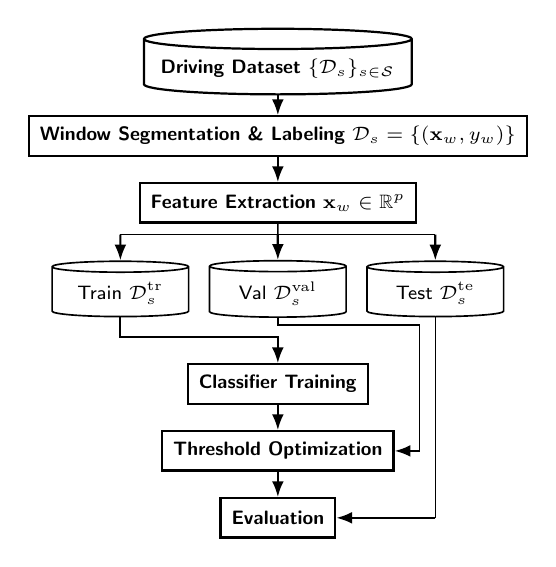
\begin{tikzpicture}[
  every node/.style={font=\sffamily\scriptsize},
  >=Latex,
  db/.style={draw, thick, cylinder, cylinder uses custom fill,
    cylinder body fill=white, shape border rotate=90, aspect=0.08,
    minimum width=3.4cm, minimum height=0.7cm, align=center,
    font=\sffamily\scriptsize},
  dbsm/.style={draw, semithick, cylinder, cylinder uses custom fill,
    cylinder body fill=white, shape border rotate=90, aspect=0.08,
    minimum width=1.7cm, minimum height=0.5cm, text width=1.5cm,
    align=center, font=\sffamily\scriptsize},
  pbox/.style={draw, thick,
    align=center, fill=white,
    minimum height=0.5cm,
    inner xsep=4pt, inner ysep=2pt,
    font=\sffamily\scriptsize},
  arr/.style ={-{Latex[length=2mm, width=1.5mm]}, thick},
]

%% ROW 0 — Dataset
\node[db] (dataset) at (0,0)
  {\textbf{Driving Dataset}~$\{\mathcal{D}_s\}_{s \in \mathcal{S}}$};

%% ROW 1 — Window segmentation \& labeling
\node[pbox] (label) at (0,-0.85)
  {\textbf{Window Segmentation \& Labeling}~$\mathcal{D}_s = \{(\mathbf{x}_w, y_w)\}$};
\draw[arr] (dataset.south) -- (label.north);

%% ROW 2 — Feature extraction
\node[pbox] (feat) at (0,-1.70)
  {\textbf{Feature Extraction}~$\mathbf{x}_w \in \mathbb{R}^p$};
\draw[arr] (label.south) -- (feat.north);

%% ROW 3 — Train / Val / Test split (per-subject, chronological)
\node[dbsm] (train) at (-2.0,-2.85) {Train~$\mathcal{D}_s^{\mathrm{tr}}$};
\node[dbsm] (val)   at ( 0.0,-2.85) {Val~$\mathcal{D}_s^{\mathrm{val}}$};
\node[dbsm] (test)  at ( 2.0,-2.85) {Test~$\mathcal{D}_s^{\mathrm{te}}$};

%% Fork: trunk down from Feature Extraction, then horizontal split
%% forkF is the midpoint between feat.south and val.north (exactly centred).
\coordinate (forkF) at ($(feat.south)!0.3!(val.north)$);
\draw[semithick] (feat.south) -- (forkF);
\draw[semithick] (-2.0,0 |- forkF) -- (2.0,0 |- forkF);
\draw[arr] (-2.0,0 |- forkF) -- (train.north);
\draw[arr] ( 0.0,0 |- forkF) -- (val.north);
\draw[arr] ( 2.0,0 |- forkF) -- (test.north);

%% ROW 4 — Classifier Training
\node[pbox] (cls) at (0,-4.00)
  {\textbf{Classifier Training}};
\draw[arr]
  (train.south) -- ++(0,-0.25) -| (cls.north);

%% ROW 5 — Threshold Optimization
\node[pbox] (thr) at (0,-4.85)
  {\textbf{Threshold Optimization}};
\draw[arr] (cls.south) -- (thr.north);

%% ROW 6 — Evaluation
\node[pbox] (eval) at (0,-5.70)
  {\textbf{Evaluation}};
\draw[arr] (thr.south) -- (eval.north);

%% ============================================================
%% Auxiliary side branches (val -> threshold; test -> evaluation).
%%   - Val  trunk: right to x=+2.2, vertical to thr level (y=-4.65)
%%   - Test trunk: straight down from test.south (x=+3.0) to eval level (y=-5.60)
%% val_horiz (y=-2.95) lies below train/val/test box south (~y=-2.80);
%% val_vert (x=2.2) never crosses test_vert (x=3.0).
%% ============================================================
%% Val trunk -> Threshold Optimization
\draw[semithick]
  (val.south) -- (0.0,-3.25) -- (1.8,-3.25) -- (1.8,-4.85);
\draw[arr] (1.8,-4.85) -- (thr.east);

%% Test trunk -> Evaluation (straight down from test.south)
\draw[semithick] (test.south) -- (2.0,-5.70);
\draw[arr] (2.0,-5.70) -- (eval.east);

\end{tikzpicture}
\end{document}
